% Scalar instruction entry source: tools/generate_scalar_instruction_catalog.py.
\subsection{\texttt{EBREAK}}
\label{sec:scalar-ebreak}
\index{EBREAK@\texttt{EBREAK}}
\begin{sloppypar}\noindent\textbf{Purpose.} Execution-control instruction used for debugging, ordering, or bring-up.\end{sloppypar}\smallskip
\noindent\textbf{Syntax.}\par
\begin{lstlisting}[style=ptoscalarcode]
ebreak imm
\end{lstlisting}
\noindent\textbf{Encoding.}\par
\noindent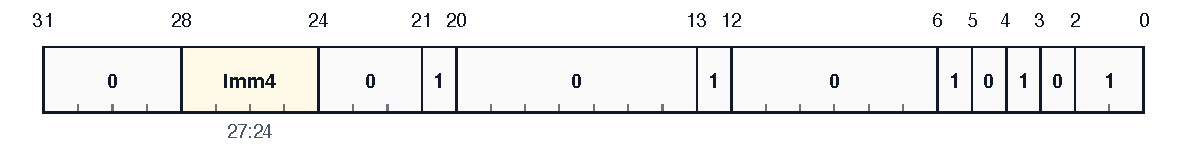
\includegraphics[width=\textwidth]{figs/encoding/scalar_instruction_entries/enc_ebreak.pdf}\par\smallskip
\begin{description}[leftmargin=0.18\linewidth,style=nextline]
\item[Format] \texttt{L32} \texttt{32-bit} scalar word.
\item[Pattern] \texttt{0000....000100000001000000101011}.
\end{description}
\noindent\textbf{Classification.}\par
\begin{description}[leftmargin=0.18\linewidth,style=nextline]
\item[Category] System, Cache, SSR, and Execution Control.
\item[Family] Execution Control.
\item[Execution class] \texttt{SYS}; uop\_kind=SYS.
\end{description}
\noindent\textbf{Operand fields.}\par
\begin{description}[leftmargin=0.18\linewidth,style=nextline]
\item[\texttt{imm4}] Bits \texttt{27:24 (4b)}. 4-bit unsigned immediate operand consumed directly by the operation.
\end{description}
\noindent\textbf{Operation.}\par
\begin{lstlisting}[style=ptoscalarcode]
Trap(SW_BREAKPOINT)
\end{lstlisting}
\Needspace{0.08\textheight}
